% Niveau :      PC
% Discipline :  Mécaflu
%Mots clés :    Viscosité, Couche limite, Equation de Blasius

\begin{exercise}{Anticyclones et dépressions}{3}{Spé}
{Mécanique des fluides, Mécanique en référentiel non galiléen, Fluide géostrophique}{bermu}

Le but de cet exercice est d'aborder la dynamique de l'atmosphère à la surface de la Terre à l'échelle globale. On se place dans le référentiel terrestre en rotation à la vitesse $\vOm = \Omega\ve_z$.

\DeclareNonDimensionalNumber{R}{o} %Rossby

\begin{questions}
    \questioncours Quelles sont les différences forces volumiques qui s'appliquent à un fluide à la surface de la Terre ? Exprimer notamment le terme d'inertie d'entraînement sous forme de potentiel.
    \question\label{que:rossby} En interprétant le nombre de Rossby 
    $$\RoN = \dfrac{v}{2L\Omega\cos\theta}$$
    et en l'estimant pour l'atmosphère, justifiez que l'équation de Navier--Stockes puisse se simplifier ainsi
    $$\pdv{\vv}{t} + 2\vOm\cross\vv = -\grad\qty(\dfrac{p}{\rho} + \Phi) + \nu\grad^2\vv,$$
    où $\Phi(r)$ est un potentiel dont on donnera la cause physique et l'expression.
    \question On s'intéresse aux courants géostrophiques qui sont de basse fréquence et de viscosité négligeable.
    \begin{parts}
        \part Quel est l'ordre de grandeur des fréquences concernées ?
        \part Justifier que la composante ascensionnelle de la vitesse ($v_r$) est négligeable.
        \part\label{que:buys} Montrer la loi de Buys--Ballot :
        
            \quad\begin{minipage}{15cm}
            \itshape i. Dans l'hémisphère nord, si on se place dos au vent, il y aura une dépression à notre gauche et un anticyclone à notre droite ; et inversement dans l'hémisphère sud. \\
            ii. En suivant ainsi le vent, il subira toujours la même pression.
            \end{minipage}
        \part Interpréter ces résultats sur les vents géostrophiques en termes météorologiques à l'aide de la figure ci dessous.
    \end{parts}
    \end{questions}
\begin{EnvUplevel}
\begin{figure}[H]
    \centering
    \vspace{-1em}
    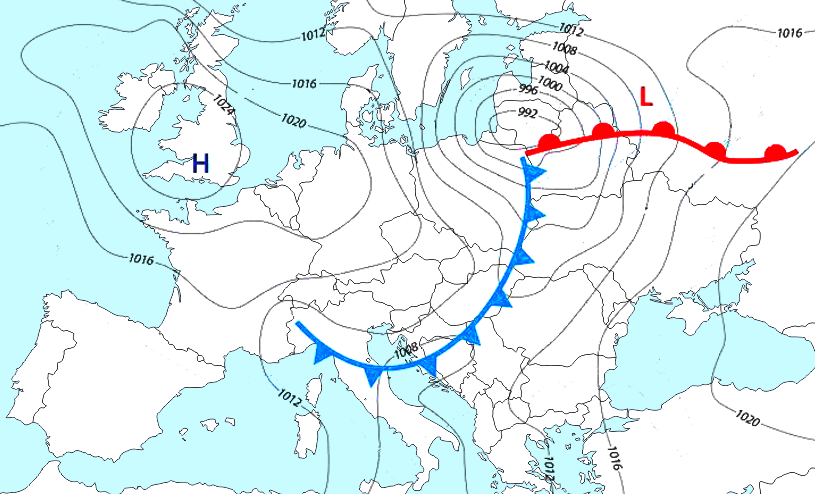
\includegraphics[width=0.9\linewidth]{mecaflu/meteo.png}
    \caption{Carte de fronts et d'isobares météo en Europe du 5 Juillet 2018.}
    \label{fig:my_label}
\end{figure}
\end{EnvUplevel}

\begin{center}
    \vspace{-1.5em}
    \itshape --- \quad Suite au verso \quad ---
\end{center}
\end{exercise}

\pagebreak

\printexerciseheader

\begin{center}
    \itshape --- \quad Suite du recto \quad ---
\end{center}

\bigskip

\begin{questions}
\setcounter{question}{3}
    \question On s'intéresse à présent aux effets de viscosité sur les vents géostrophiques. Pour simplifier, on va supposer que nous sommes en Europe où la latitude est environ de 45$^\circ$ N.
    \begin{parts}
        \part Estimer la valeur du nombre de Reynolds $\ReN$. Dans quelles régions les effets visqueux vont être prédominants ?
        \part Considérant que nous sommes en 2D et en utilisant le résultat \emph{ii.} de la question \ref{que:buys}, projeter l'équation précédente suivant les isobares horizontales et dans la direction perpendiculaire.
        \part Par un changement de variable complexe, monter que la viscosité à pour effet que la vitesse au sol fait un angle à 45$^\circ$ (sans rapport avec la latitude) par rapport aux isobares et qu'elle s'oriente vers ces dernières avec l'altitude en faisant une spirale.
        \part Donner l'altitude caractéristique $\delta$ de cette couche visqueuse et conclure par rapport au cas précédent.
    \end{parts}
\end{questions}

\plusloin
Il existe également des phénomènes ondulatoires appelés ondes inertielles que l'on peut déduire de l'équation de la question \ref{que:rossby}.

En outre les phénomènes météorologiques sont étroitement liés à la convection thermique entre les zones équatoriales où il fait chaud et les zones polaires où il fait froid.